%%%%%%%%%%%%%%%%%%%%%%%%%%%%%%%%%%%%%%%%%
% a0poster Portrait Poster
% LaTeX Template
% Version 1.0 (22/06/13)
%
% The a0poster class was created by:
% Gerlinde Kettl and Matthias Weiser (tex@kettl.de)
% 
% This template has been downloaded from:
% http://www.LaTeXTemplates.com
%
% License:
% CC BY-NC-SA 3.0 (http://creativecommons.org/licenses/by-nc-sa/3.0/)
%
%%%%%%%%%%%%%%%%%%%%%%%%%%%%%%%%%%%%%%%%%

%----------------------------------------------------------------------------------------
% PACKAGES AND OTHER DOCUMENT CONFIGURATIONS
%----------------------------------------------------------------------------------------

\documentclass[a0,portrait]{a0poster}

\usepackage{multicol} % This is so we can have multiple columns of text side-by-side
\columnsep=100pt % This is the amount of white space between the columns in the poster
\columnseprule=3pt % This is the thickness of the black line between the columns in the poster

\usepackage[svgnames]{xcolor} % Specify colors by their 'svgnames', for a full list of all colors available see here: http://www.latextemplates.com/svgnames-colors

\usepackage{times} % Use the times font
%\usepackage{palatino} % Uncomment to use the Palatino font

\usepackage{float}
\usepackage{graphicx} % Required for including images
\graphicspath{{figures/}} % Location of the graphics files
\usepackage{booktabs} % Top and bottom rules for table
\usepackage[font=small,labelfont=bf]{caption} % Required for specifying captions to tables and figures
\usepackage[utf8]{inputenc}
%\usepackage[slovene,english]{babel}
\usepackage{amsfonts, amsmath, amsthm, amssymb} % For math fonts, symbols and environments
\usepackage{wrapfig} % Allows wrapping text around tables and figures
\usepackage{lipsum}

\begin{document}

%----------------------------------------------------------------------------------------
% POSTER HEADER 
%----------------------------------------------------------------------------------------

% The header is divided into two boxes:
% The first is 75% wide and houses the title, subtitle, names, university/organization and contact information
% The second is 25% wide and houses a logo for your university/organization or a photo of you
% The widths of these boxes can be easily edited to accommodate your content as you see fit

\begin{minipage}[b]{1\linewidth}
\veryHuge \color{Black} \textbf{Dinaric Karst Dolines - A Case Study of Menišija, Slovenia} \color{Black}\\ % Title
%%\Huge\textit{Case Study of Menišija, Slovenia}\\[1cm] % Subtitle
\centering
\Large \textbf{Rok Mihevc}, rok@mihevc.org, Grič 10, Logatec, Slovenia % Author(s)
%\huge University of Ljubljna, Faculty of Mathematics and Physics\\[0.4cm] % University/organization
%%\Large \texttt{rok@mihevc.org}
\end{minipage}
%
\vspace{1cm} % A bit of extra whitespace between the header and poster content

%----------------------------------------------------------------------------------------

\begin{multicols}{2} % This is how many columns your poster will be broken into, a portrait poster is generally split into 2 columns

%----------------------------------------------------------------------------------------
% ABSTRACT
%----------------------------------------------------------------------------------------

%\color{Navy} % Navy color for the abstract

\begin{abstract}

Dolines are a frequent karst feature. Their shape, genesis and dynamics are conceptually described by various models. However, to the author’s knowledge there was no data about exact shape and size of a larger set of karst dolines that could be used for statistical analysis.
We developed and used a numerical method to analyze $60 km^2$ of $1 m$ grid resolution lidar data of digital relief model of Menišija, a levelled karst surface, former polje near Postojna, Slovenia. We identified $8.700$ dolines (about $145$ dolines$/ km^2$). We then used numerical tools to calculate the average shape of the identified dolines and proposed a function to describe this shape.

Due to the geological history of Menišija and similarity of dolines in the area we propose that they were shaped by the same geomorphological processes, that ultimately lead to a common geomorphologically stable form of doline which is already reached in this area. 

Using this hypothesis we propose two possible dynamical models for dolines that would lead to the shape of relief that we observe in Menišija today.
\end{abstract}

%----------------------------------------------------------------------------------------
% INTRODUCTION
%----------------------------------------------------------------------------------------

%%\color{SaddleBrown} % SaddleBrown color for the introduction

\section*{About Dinaric dolines}
\begin{wrapfigure}{r}{0.2\textwidth}
\begin{center}
  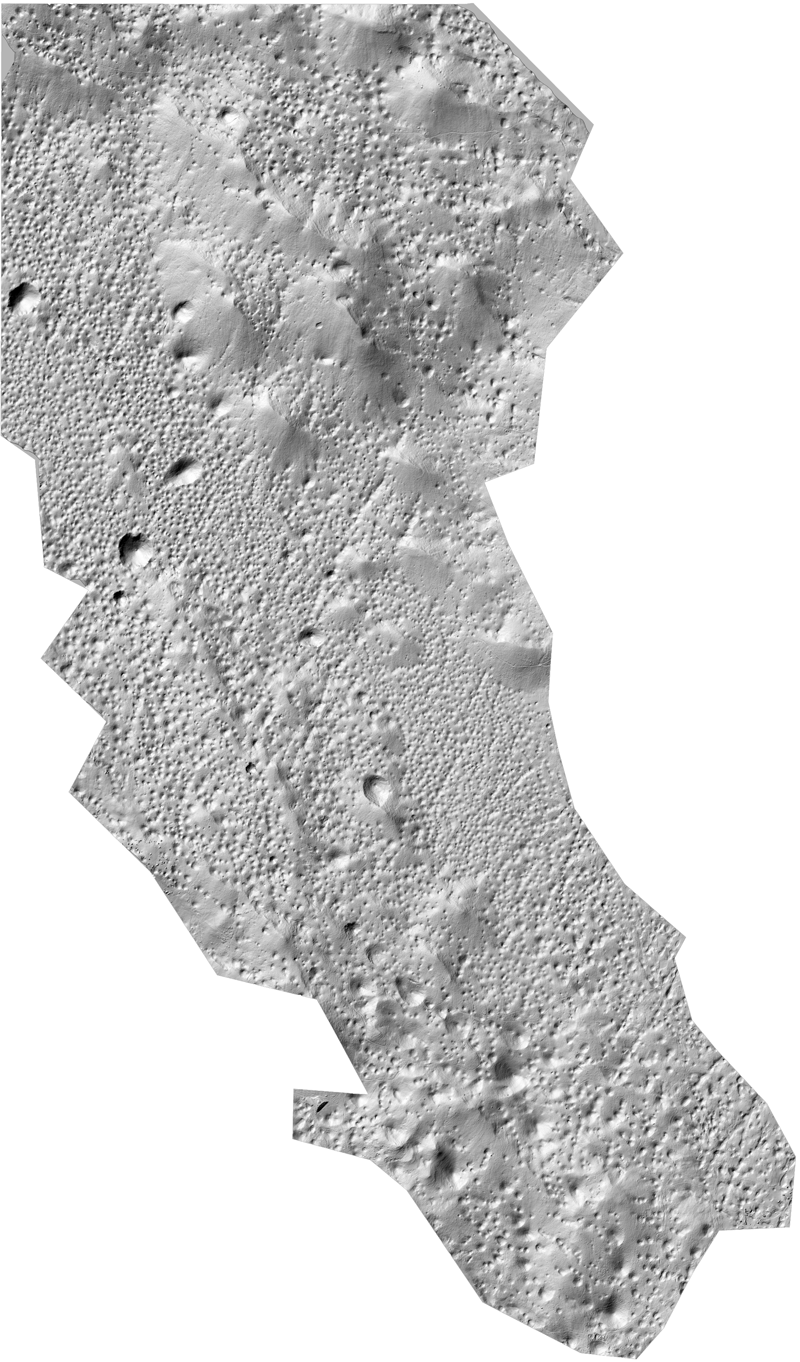
\includegraphics[width=0.2\textwidth]{menisija-relief.png}
  \captionof{figure}{Shaded digital model of Menišija.}
  \label{fig:menisija}
\end{center}
\end{wrapfigure}
Dolines of Classical karst are closed, bowl shaped depression with diameter ranging from about 10 to 100 meters. While each doline has its specific history, we can notice similarities in size and shape of dolines found in the same region. This leads us to believe, that no matter the history, they are ultimately shaped by the same process. This conclusion gives motivation for the presented study.

It is believed that predominant factor of genesis and growth of dolines is chemical dissolution of limestone (\cite{ford2007karst}, \cite{Zambo1997}). The dissolved limestone is washed into the aquifer trough fractures in the bedrock, while the surface is lowered and fractures widened. Deepening of the dolines may cause further concentration of surface water and also trigger other mechanisms (soil concentration, $CO_2$ production, etc.), that further enhances dissolution of limestone. A feedback loop is established that drives the growth of the doline. However the growth is not unbound, as all dolines eventually reach a stable, adult, form that we most commonly observe in nature. We assume this is caused by creation of efficient drainage system in the doline, that minimizes the dissolution of limestone, locking the dissolution of doline surface in step with adjacent flat surface.

To study a statistically relevant set of dolines we used a high resolution digital relief model provided by Slovenian Forestry Institute \cite{LAK}, \cite{Kobler20079}.

%----------------------------------------------------------------------------------------
% OBJECTIVES
%----------------------------------------------------------------------------------------

%%\color{DarkSlateGray} % DarkSlateGray color for the rest of the content

\section*{Computer vision method}

To isolate dolines from the digital relief model we calculated concavity of each point in the relief by assigning the point a value calculated by subtracting the points height from the average height of points on a concentric ring around it. By varying the rings inner and outer radius we highlighted concave shapes of various sizes.
We then segmented the area into concave zones and chose the most fitting candidates for dolines.

  \begin{minipage}[b]{0.5\textwidth}
      \begin{minipage}{0.45\linewidth}
          \begin{figure}[H]
              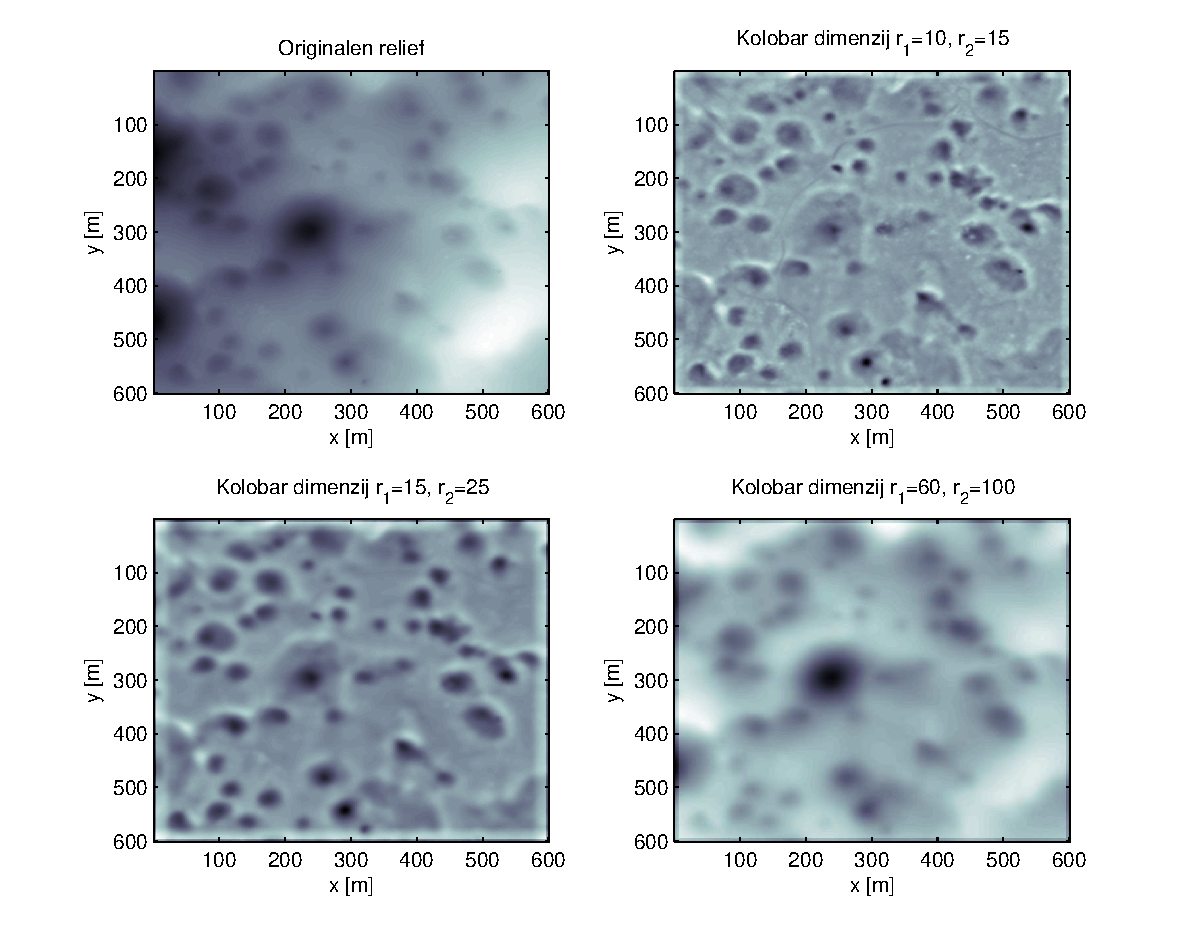
\includegraphics[width=\textwidth]{concavity-samples.pdf}
              \caption{Concavity index of relief for various ring sizes.}
              \label{fig:concavity-samples}
          \end{figure}
      \end{minipage}
      \begin{minipage}{0.45\linewidth}
          \begin{figure}[H]
              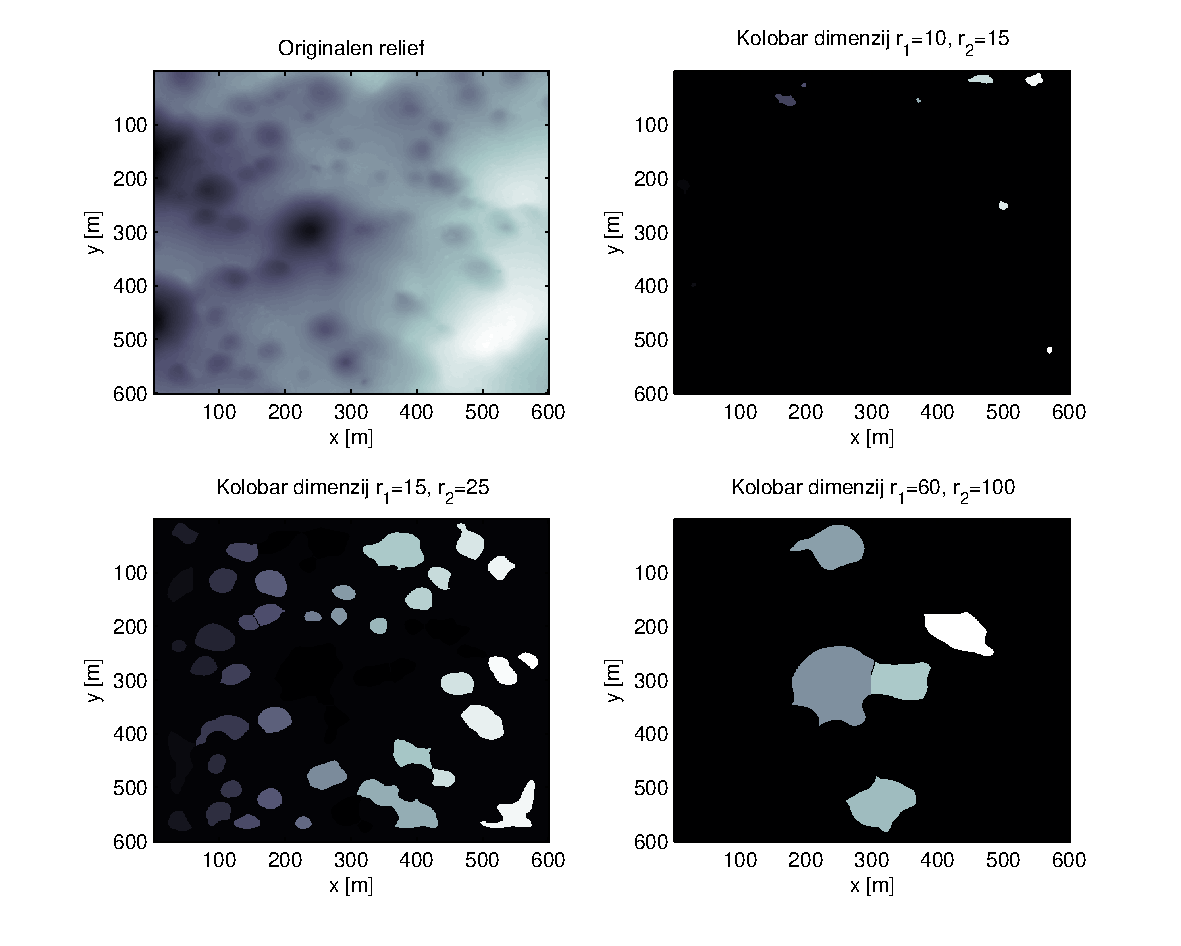
\includegraphics[width=\textwidth]{concavity-segmentation-samples.pdf}
              \caption{Segmentation based on concavity index.}
              \label{fig:concavity-segmentation}
          \end{figure}
      \end{minipage}
  \end{minipage}

%----------------------------------------------------------------------------------------
% MATERIALS AND METHODS
%----------------------------------------------------------------------------------------

\section*{Results and Analysis}

We then calculated the effective radii of found dolines, by counting the pixels of each doline and calculating the radius of a circle with equal surface (see equation (\ref{eq:reff}).

\begin{equation}
  \sum pixels = surface = \pi \cdot r^2
  \label{eq:reff}
\end{equation}

Overlay of the identified dolines and histogram of effective radii can be seen on Figure \ref{fig:vrtaceinpolmeri}.

  \begin{minipage}[b]{0.5\textwidth}
      \begin{minipage}{0.2\linewidth}
          \begin{figure}[H]
              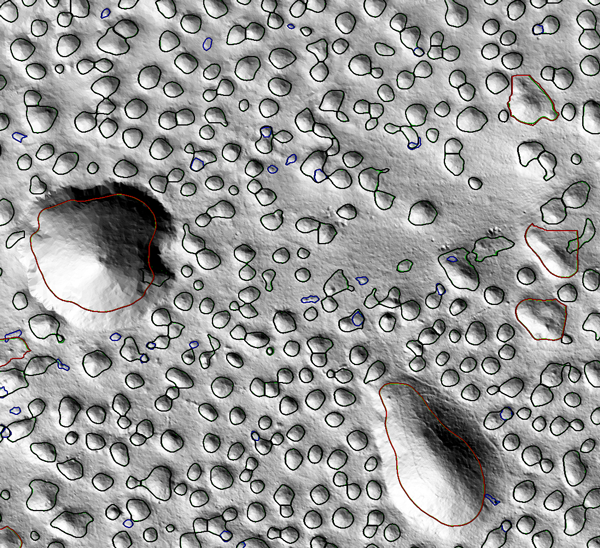
\includegraphics[width=\textwidth]{menisija-vrtace}
              \caption{Part of 8700 dolines found in the Menišija and two collapse dolines.}
              \label{fig:vrtaceinpolmeri}
          \end{figure}
      \end{minipage}
      \begin{minipage}{0.83\linewidth}
          \begin{figure}[H]
              \captionsetup{margin=2cm}
              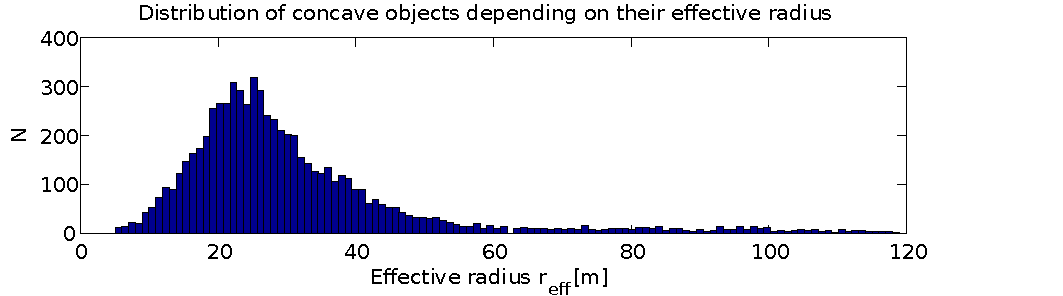
\includegraphics[width=\textwidth]{menisija-polmeri-hist-4}
              \caption{Histogram of effective radii of concave objects in Menišija. \\Average effective radius is $\overline{r_{eff}} = 26m$.}
              \label{fig:vrtave-histogram}
          \end{figure}
      \end{minipage}
  \end{minipage}

\vspace{5mm}
The effective radius of identified dolines appears to be normally distributed with a maximum at $26m$.

We proceeded by averaging all the identified dolines, to remove historical and directional bias. The result can be seen in Figure \ref{fig:vrtaca}.

To approximate the shape of the average doline we proposed an upside down Gaussian function:

\begin{equation}
  f(r) = - A \cdot e^{\frac{r^2}{\sigma^2}} + C.
  \label{eq:Gaussian}
\end{equation}

\vfill
\columnbreak
\begin{wrapfigure}{r}{0.18\textwidth}
  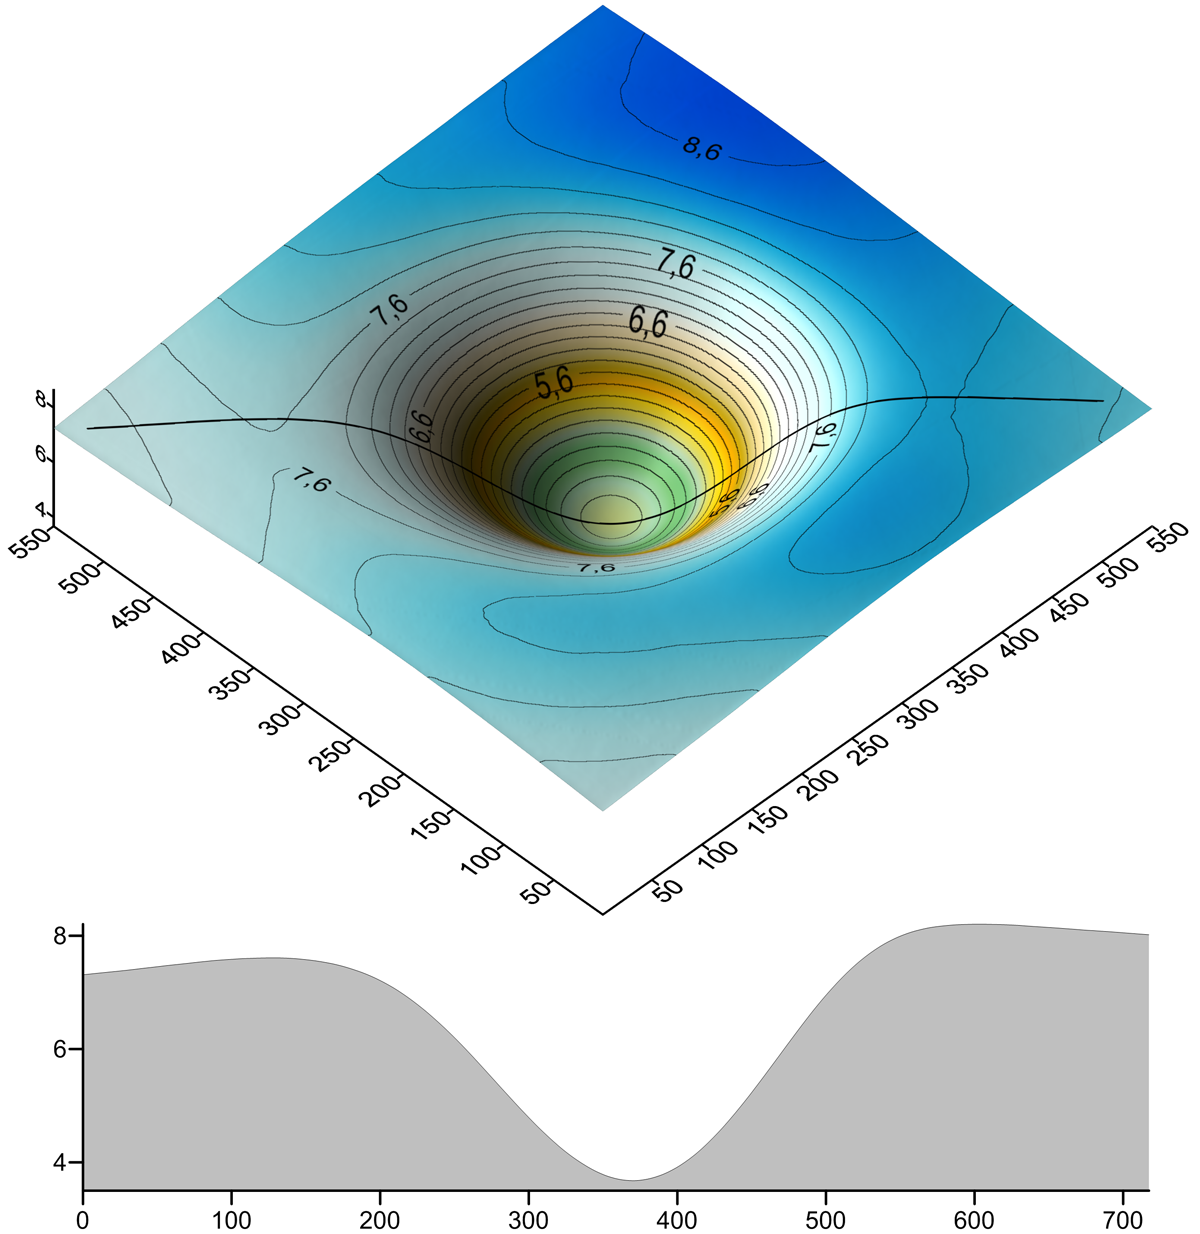
\includegraphics[width=\linewidth]{menisija-vrtaca.png}
  \captionof{figure}{Average doline of Menišija. Averaged of $8700$ dolines found.}
  \label{fig:vrtaca}
\end{wrapfigure}

To get a better idea about how similar the dolines of Menišija are to one another we now fit the proposed function (\ref{eq:Gaussian}) to identified dolines and plot the optimal fitting parameters on Figure \ref{fig:vrtace-fit}. The fitting parameters are the depth $A$ and width $\sigma$. From the area of concavity we already calculated effective radius $r_{eff}$ according to equation (\ref{eq:reff}).


The results suggest:
\begin{itemize}
  \item There is a linear correlation between $\sigma$ and $r_{eff}$, indicating proposed function (\ref{eq:Gaussian}) is good enough for describing the area of dolines.
  \item There is linear correlation between the depth $A$ and $r_{eff}$ as well as $A$ and $\sigma$, meaning the wider the doline is, the deeper it will be.
\end{itemize}

\vspace{0.7cm}
  \begin{figure}[H]
    \centering
    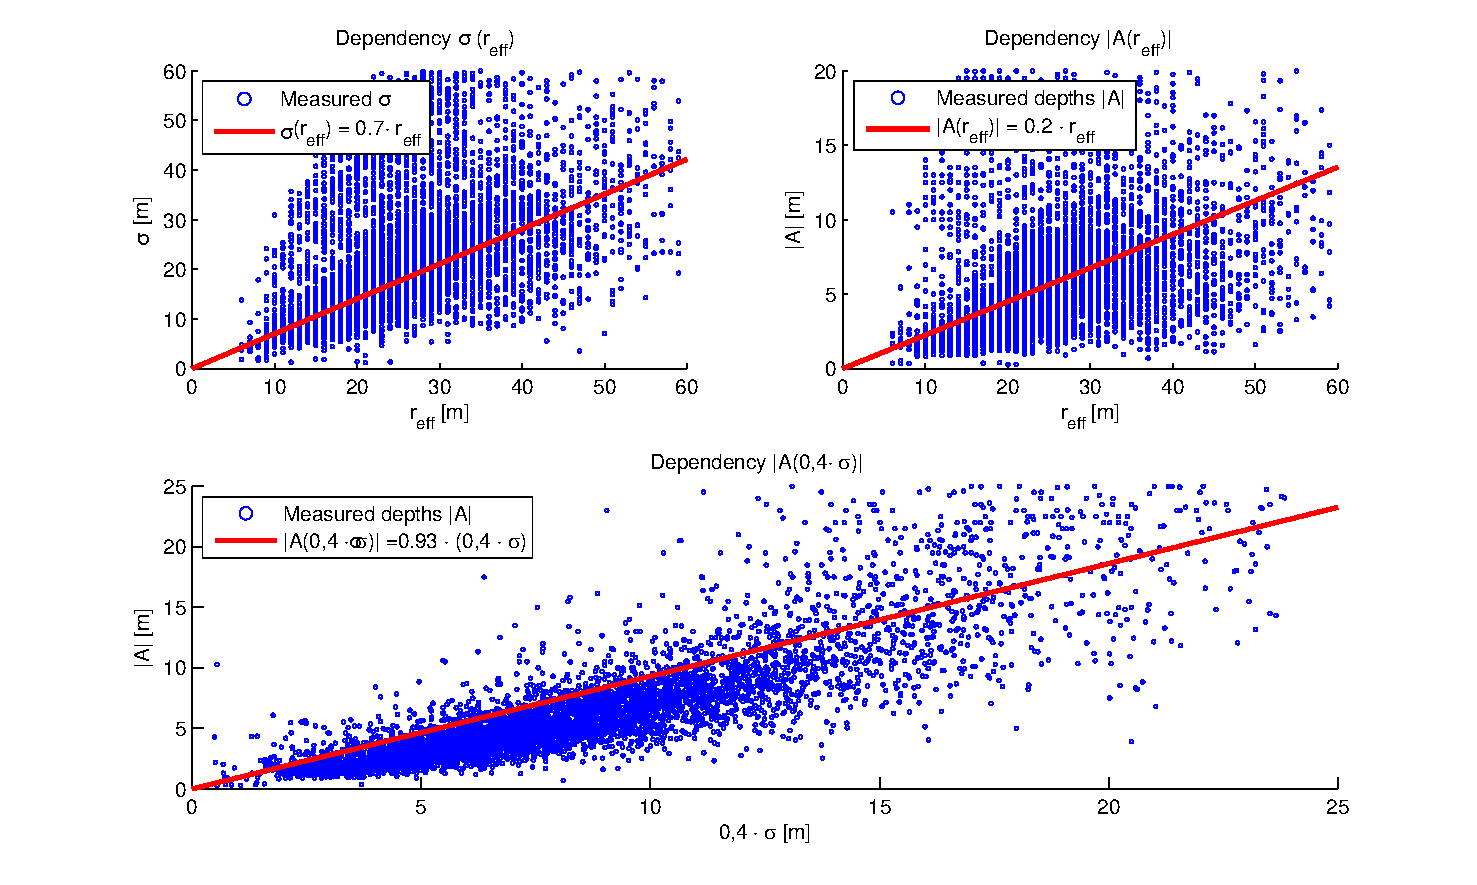
\includegraphics[width=0.85\linewidth]{menisija-A-sigma-reff-2.pdf}
    \caption{We pick dolines of typical sizes ($5m < r_{eff} < 60m$) and plot dependencies $\sigma(r_{eff})$, $A(r_{eff})$, $A(\sigma)$. We then fit linear functions onto them to show correlations.}
    \label{fig:vrtace-fit}
  \end{figure}

%----------------------------------------------------------------------------------------
% CONCLUSIONS
%----------------------------------------------------------------------------------------

\section*{Proposed dynamic model}

Menišija is levelled surface, part of former much larger karst polje. Polje was vertically fragmented to smaller parts by tectonic movements. They lowered the level of karst water and diverted the surface inflow that was flooding and levelling Menišija to the nearby Cerkniško polje. The dolines appeared in the time period from then to present. Judging by our findings about depth and size distributions, the dolines appear to have reached a stable shape and their depths and sizes stopped to develop.
This fact motivated us to study partial differential equations that take initial conditions of a flat surface and ultimately produce doline like shapes, that are stable and do not grow or diminish in time. We propose two models for this dynamic.

\vspace{5mm}
\textit{Logistic growth}
\begin{equation}
  \frac{ \partial h(\mathbf{x},t) }{ \partial t} = D \frac{\partial^2}{\partial \mathbf{x}^2} h(\mathbf{x},t) + a \cdot h(\mathbf{x},t) \cdot (1 - \frac{h(\mathbf{x},t)}{K})
  \label{eq:logistic-growth}
\end{equation}
Logistic growth equation produces a dynamics, where doline grows slowly at first, but as its size increases so does its growth rate. But, as the doline approaches the carrying capacity (see the second term in (\ref{eq:logistic-growth})), the growth diminishes and stops. Carrying capacity is defined by border conditions set by the environment.
Given border conditions:
\begin{equation}
  \begin{aligned}
    h(\mathbf{x},0) =  - e^{-\mathbf{x}^2}, \mathbf{x} \in D, \\
    h(\mathbf{x},t) = 0, \mathbf{x} \in \partial D, \\
    \mathbf{n} \cdot \boldsymbol \nabla h(\mathbf{x},t) = 0, \mathbf{x} \in \partial D,
  \end{aligned}
\end{equation}
we get a dynamics as seen on Figure \ref{fig:logistic-growth}.

\vspace{5mm}
\textit{Kardar-Parisi-Zhang}
\begin{equation} \frac{ \partial h(\mathbf{x},t)}{ \partial t} = D \nabla^2 h(\mathbf{x},t) + F(h(\mathbf{x},t)) \label{eq:kpz} \end{equation}
Kardar-Parisi-Zhang equation gives us a non-deterministic dynamic model for growth of dolines. Starting from a flat surface this model will produce a Figure \ref{fig:kpz}-like surface. The size and depth of dolines in this model will depend on the diffusion constant $D$ and stochastic term $F(h(\mathbf{x},t))$ as seen in equation (\ref{eq:kpz}).

  \begin{minipage}[b]{0.5\textwidth}
  \centering
      \begin{minipage}{0.43\linewidth}
          \begin{figure}[H]
              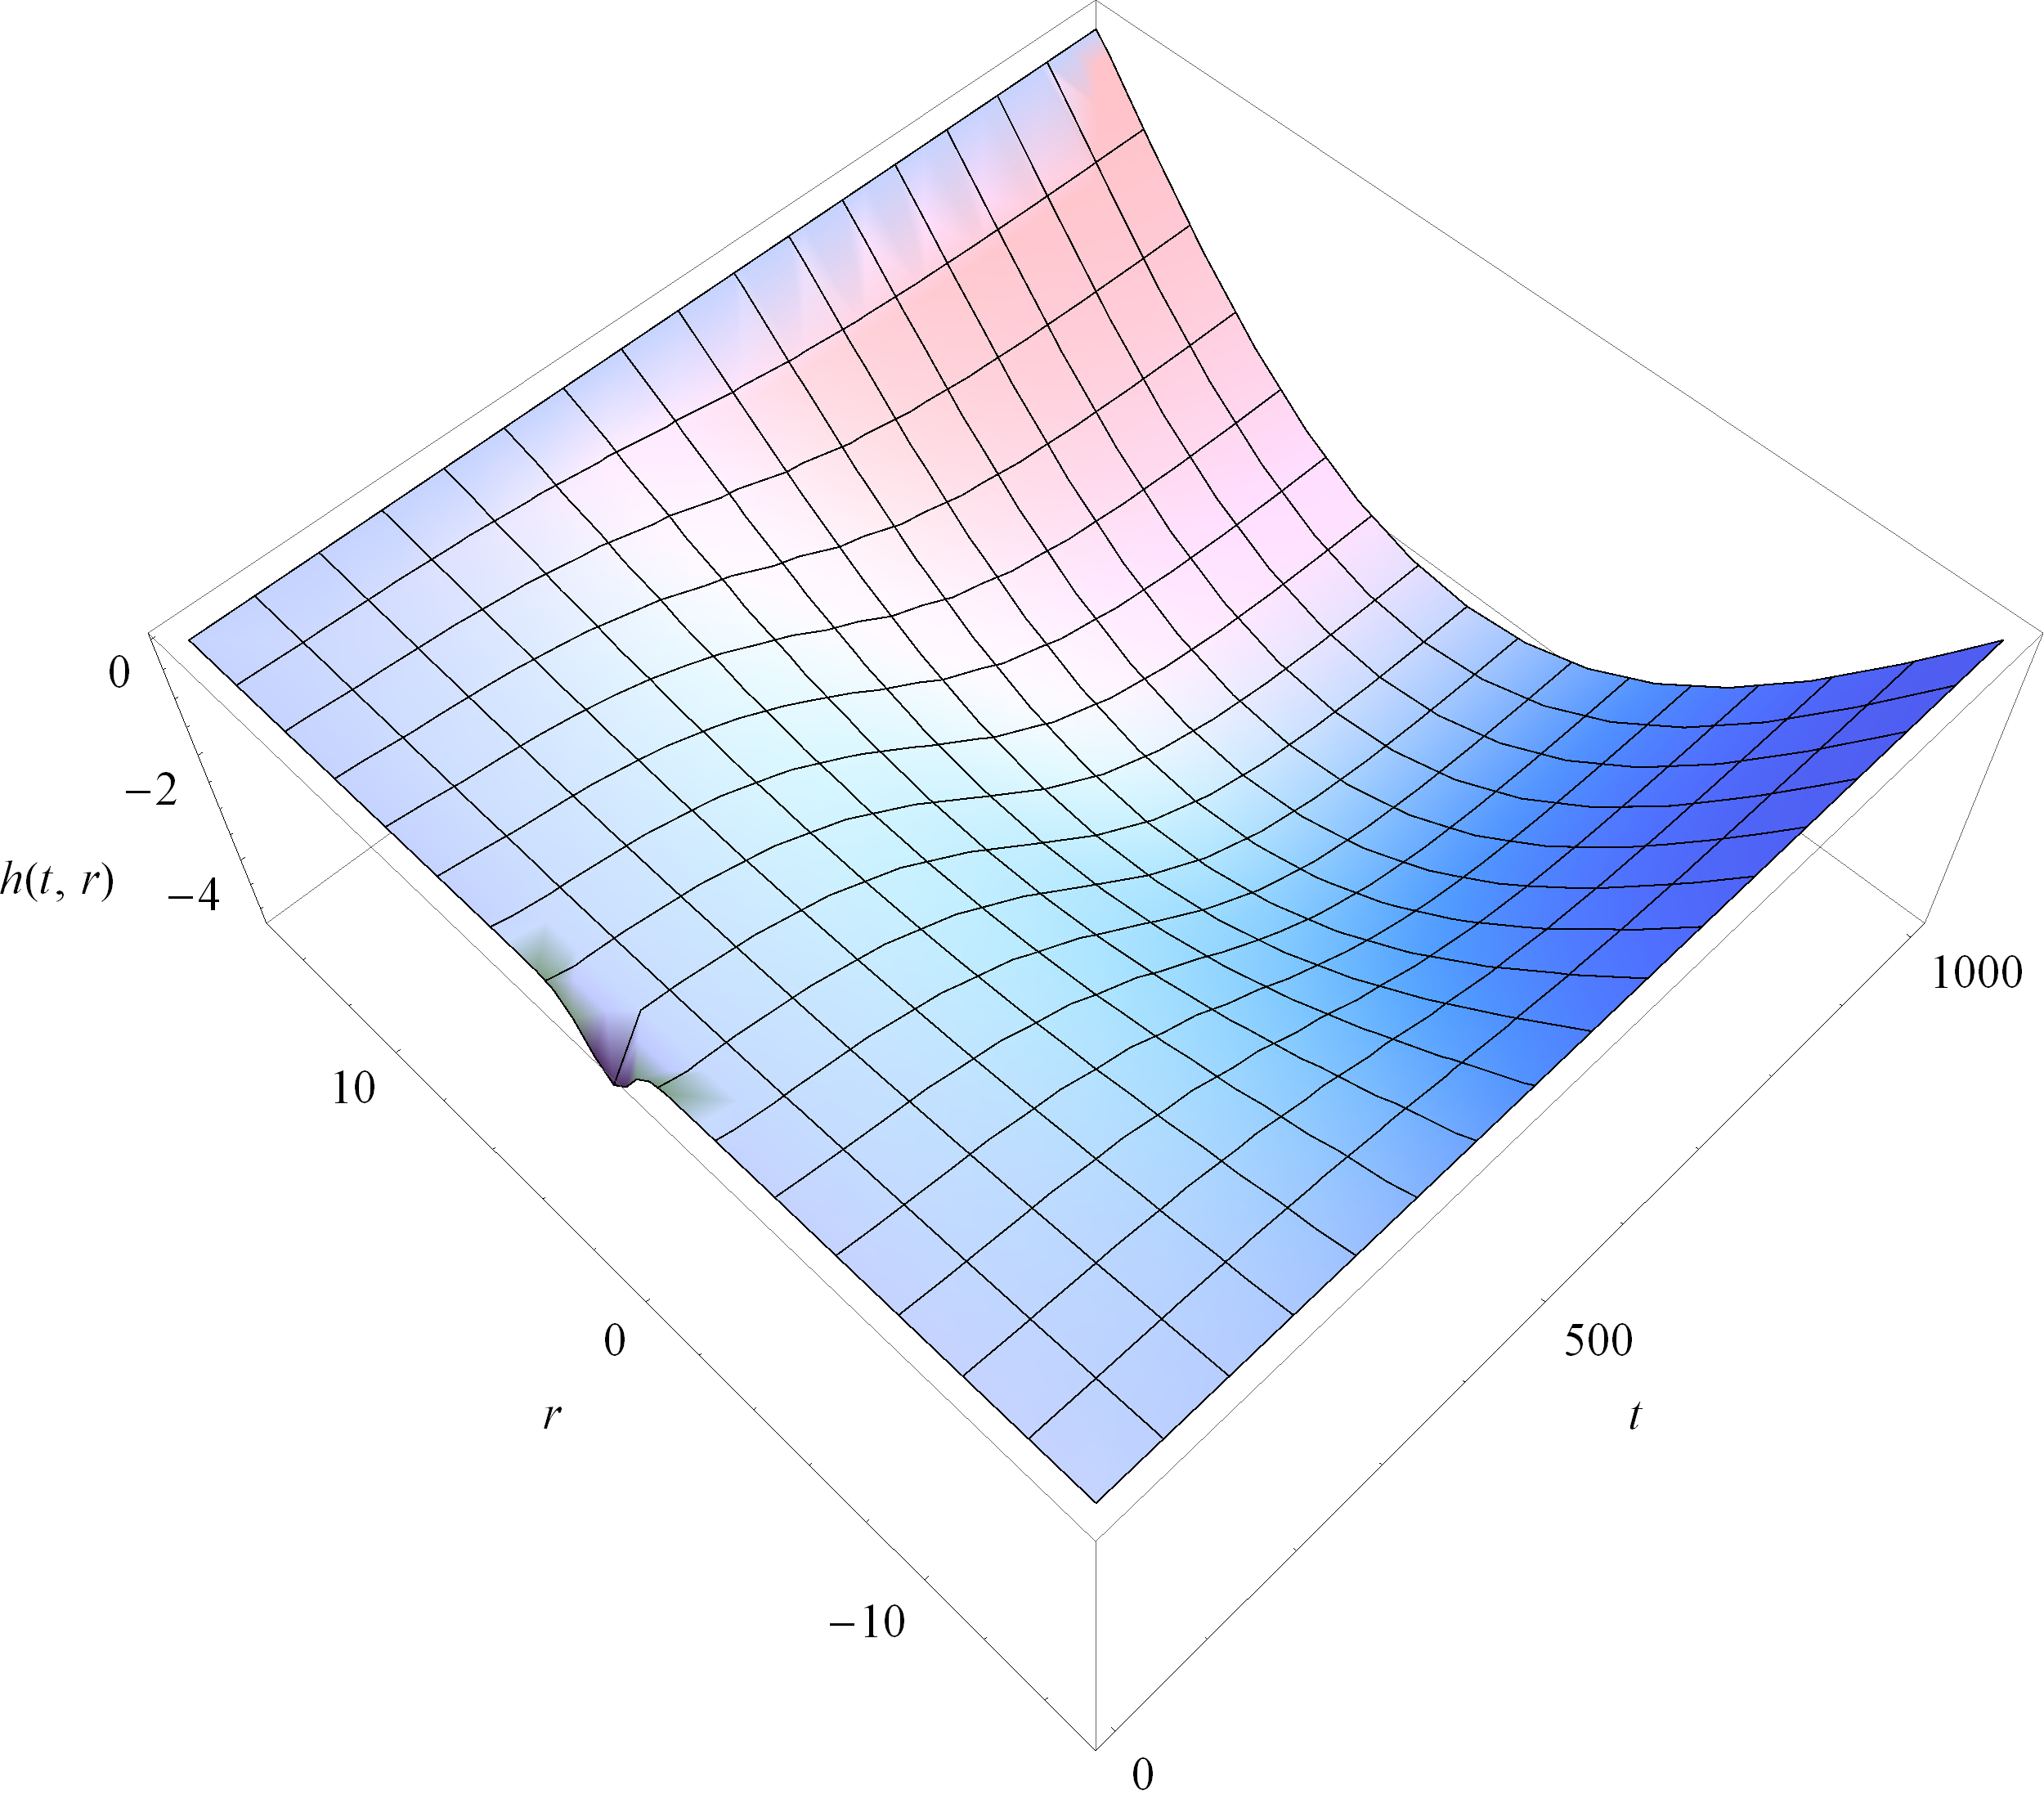
\includegraphics[width=\textwidth]{difuzija-logisticna-rast2.png}
              \caption{Time evolution of logistic diffusion growth given by equation (\ref{eq:logistic-growth}). We set $D = 1$, $a = 50$, $K = -10$.}
              \label{fig:logistic-growth}
          \end{figure}
      \end{minipage}
      \hspace{0.05\linewidth}
      \begin{minipage}{0.5\linewidth}
          \begin{figure}[H]
              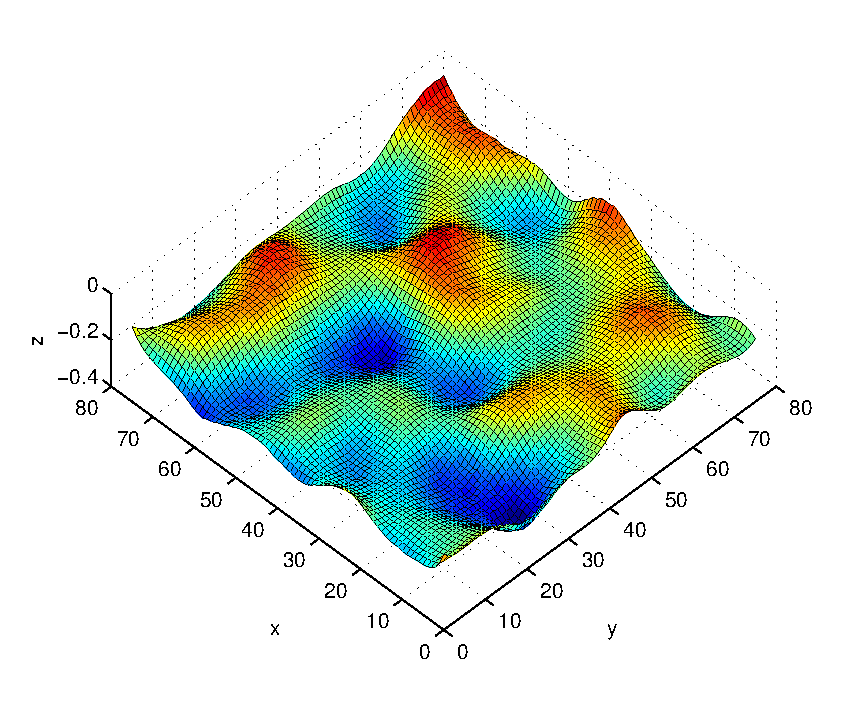
\includegraphics[width=\textwidth]{KPZ-numericno.pdf}
              \caption{Final result of numeric simulation of Kardar-Parisi-Zhang dynamics, starting from a flat surface after $10^5$ steps.}
              \label{fig:kpz}
          \end{figure}
      \end{minipage}
  \end{minipage}

%%\color{SaddleBrown} % SaddleBrown color for the conclusions to make them stand out
% \color{DarkSlateGray} % Set the color back to DarkSlateGray for the rest of the content

%----------------------------------------------------------------------------------------
% REFERENCES
%----------------------------------------------------------------------------------------

\nocite{*} % Print all references regardless of whether they were cited in the poster or not
\bibliographystyle{plain} % Plain referencing style
\bibliography{references} % Use the example bibliography file sample.bib

\end{multicols}
\end{document}